\documentclass[conference]{IEEEtran}
\usepackage[utf8]{inputenc}
\usepackage[T1]{fontenc}
\usepackage{graphicx}
\usepackage{booktabs}
\usepackage{amsmath}
\usepackage{url}
\usepackage[hidelinks]{hyperref}
\usepackage{xcolor}

\begin{document}

\title{Code-Enforced Guardrails Let Small Local Language Models Operate Validated Production Simulation Models: A Held-Out Evaluation}

\author{\IEEEauthorblockN{Han Yu}
\IEEEauthorblockA{M.Eng. Applied AI for Digital Production Management\\
Technische Hochschule Deggendorf, Campus Cham, Germany\\
han.yu@stud.th-deg.de}}

\maketitle

\begin{abstract}
Discrete-event simulation answers what-if questions in production planning, but operating a validated model correctly (valid inputs, enough replications, confidence intervals, fair comparisons) requires a simulation expert. Language models can translate a planner's question into a scenario, yet they cannot verify their own steps. We present Planner Copilot, an open-source system in which a small local language model only chooses tools and parameter values, while a check engine written in code decides whether an answer can be trusted. The engine reads one case card per published simulation model and applies five checks on every call: scope, units and plausibility, validated range, adaptive replications to a 95\,\% confidence interval, and paired comparison with common random numbers. We reproduce four published models from four industries and evaluate three local models (Qwen~2.5~7B, Llama~3.1~8B, Gemma~2~9B) in three setups (no checks, rules written into the prompt, code-enforced checks) on 40 sealed test questions written after the rules were frozen. Code-enforced checks raise correct answers from 22/14/15 to 37/27/30 of 40 compared with prompt rules (exact McNemar, Holm-adjusted $p \le 0.003$ for all three models). Confidently wrong answers fall from 7/14/12 to 3/11/8, but this reduction is not significant at 40 questions. The remaining errors are out-of-scope questions that a keyword-based scope check misses and a unit conversion the engine does not check.
\end{abstract}

\begin{IEEEkeywords}
discrete-event simulation, large language models, guardrails, LLM-Modulo, production planning, verification and validation
\end{IEEEkeywords}

\section{Introduction}
A production planner faces questions such as ``a busy week with 20\,\% more orders and one worker absent: how much overtime?'' A validated discrete-event simulation (DES) model can answer them, but only when it is operated correctly: inputs must lie in the range the model was validated for, stochastic output needs enough replications for a confidence interval, and two scenarios must be compared fairly \cite{law2015,sargent2013}. Small and medium-sized enterprises rarely employ the simulation expert who knows these rules, and large companies queue such requests behind their experts.

Language models (LLMs) are an obvious interface, but auto-regressive LLMs cannot reliably plan or verify their own steps; Kambhampati et al.\ argue for LLM-Modulo frameworks in which the model proposes and external, model-based critics verify \cite{kambhampati2024}. Recent work on LLMs and manufacturing simulation mostly targets model \emph{generation} or \emph{adaptation} with frontier cloud models and human checkpoints \cite{schmitt2026,korth2026}. This paper addresses the complementary task of \emph{operating} an existing, validated model, and asks whether code that encodes simulation methodology can replace the expert checkpoint for small local models that keep production data on premises.

Contributions: (i) an architecture in which a case card (one YAML file per published model) and a model-independent check engine enforce scope, units, validity range, replication and comparison rules, while the LLM only selects tools and values; (ii) four published DES models from four industries, each reproduced against the authors' results before any question is asked; (iii) a pre-registered held-out evaluation of three local LLMs in three setups that separates the effect of the rules from the effect of enforcing them in code.

\section{Related Work}
\emph{LLMs and manufacturing DES.} Schmitt et al.\ generate, adapt and evaluate SimPy models with a fixed chain of LLM roles, two mandatory human checkpoints and closed models \cite{schmitt2026}. Korth et al.\ combine optimization, DES and an LLM agent to support workforce planning \cite{korth2026}. A concurrent preprint lets a general agent operate an open 3D simulator and validates behaviour against reference models on held-out tasks \cite{agenticdes2026}. These works rely on human review or on an LLM inspector; we move verification into deterministic code and evaluate open-weight models only.

\emph{Guardrails.} NeMo Guardrails adds programmable rails to conversational systems, mainly for topical and safety control \cite{rebedea2023}. Our rails govern numerical validity instead: they decide which simulation calls are admissible and which statistics an answer needs.

\emph{Verification and validation.} A simulation model is valid only for the experimental conditions under which it was validated \cite{sargent2013}; output analysis requires replications and confidence intervals, and comparisons benefit from common random numbers \cite{law2015}. The check engine turns these offline expert rules into checks that run on every call.

\section{System}
\begin{figure}[t]
\centering
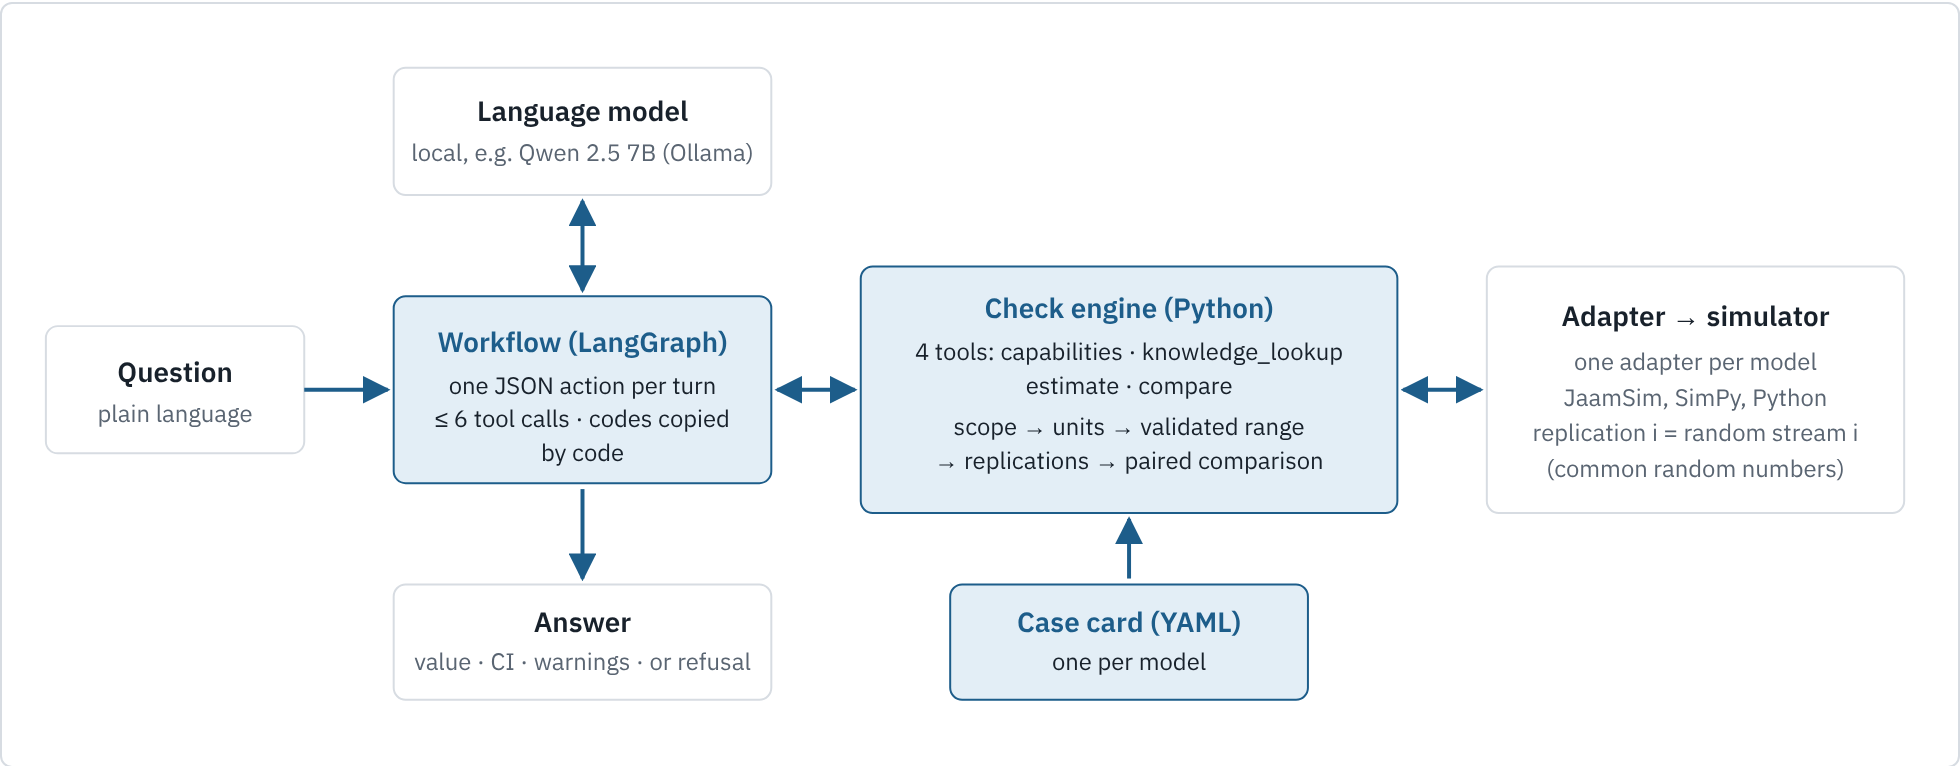
\includegraphics[width=\columnwidth]{architecture.png}
\caption{Architecture. The LLM returns one JSON action per turn (a tool call or a final answer). Code runs the tool, copies warning codes into the answer and stops after at most six tool calls. The check engine reads the case card of the selected model and calls the simulator through a per-model adapter.}
\label{fig:arch}
\end{figure}

Fig.~\ref{fig:arch} shows the three parts. The \emph{case card} records, per model, every parameter with unit, hard physical bounds and validated range; every output (KPI) with its required precision; and what the model cannot answer, as a list and as refusal keywords. The \emph{check engine} offers four tools (\texttt{capabilities}, \texttt{knowledge\_lookup}, \texttt{estimate}, \texttt{compare}) and applies five checks in order (Table~\ref{tab:checks}). The \emph{workflow} (LangGraph) asks the LLM for one JSON action per turn, which small models follow more reliably than native tool calling, and additionally checks that the number in the final answer is one the simulation returned (\texttt{value\_not\_from\_tool}). The warning codes (\texttt{outside\_valid\_range}, \texttt{precision\_not\_reached}, \texttt{not\_distinguishable}) are fixed strings copied by code, so the LLM can neither add nor drop a warning.

\begin{table}[t]
\caption{Checks applied by the engine on every simulation call}
\label{tab:checks}
\centering\small
\begin{tabular}{@{}p{0.22\columnwidth}p{0.46\columnwidth}p{0.24\columnwidth}@{}}
\toprule
Check & Rule & If violated \\
\midrule
1 Scope & KPI and parameter names exist; no refusal keyword in the question & refusal \\
2 Units & numeric; converted (min--h, \%--fraction); within hard bounds & error with hint; LLM may retry \\
3 Validity & value inside the validated range & runs, with warning \\
4 Replications & add 10 until 95\,\% CI half-width $\le$ 1\,\% of mean or KPI precision; cap 100 & warning \\
5 Paired comparison & common random numbers until the CI of the difference excludes 0 & verdict ``not distinguishable'' \\
\bottomrule
\end{tabular}
\end{table}

\section{Simulation Models}
Each case is a model published with results by its authors and reproduced before any question was written (Table~\ref{tab:cases}), so later differences cannot stem from a setup error.

\begin{table}[t]
\caption{Published models and their reproduction}
\label{tab:cases}
\centering\small
\begin{tabular}{@{}p{0.08\columnwidth}p{0.36\columnwidth}p{0.48\columnwidth}@{}}
\toprule
Case & Model & Reproduction \\
\midrule
A1 & Semiconductor fab, SMT2020 \cite{kopp2020}, simulator of \cite{tassel2023} & 28 of 28 published values within tolerance \\
A2 & Sheet-metal job shop, 69 real orders, JaamSim \cite{jurczyk2026} & identical to all 30 published replications \\
A3 & Pallet warehouse with reach trucks, SimPy \cite{saengphueng2026} & 360 of 360 published KPI means identical \\
A5 & Operator-paced assembly line, SimPy rebuild of \cite{seppanen2005} & inside the published 95\,\% CIs \\
\bottomrule
\end{tabular}
\end{table}

\section{Evaluation Method}
\emph{Setups.} A: the LLM calls the simulator directly with all checks off. B: as A, plus the same rules written as text into the system prompt (generated from the case cards). C: the LLM uses the check engine. B versus C isolates the effect of enforcing the rules in code.

\emph{Questions and grading.} Four question types: numeric (a KPI value), choice (e.g.\ which scenario is better), flag (the input lies outside the validated range, so the answer must carry \texttt{outside\_valid\_range}) and scope (the model cannot answer, so the system must refuse). A numeric answer is correct inside the tolerance (the wider of $\pm$5\,\% and $\pm$2 standard deviations of the reference). Every answer is graded \emph{correct}, \emph{cautious} (no number, or a wrong number carrying a warning) or \emph{confidently wrong} (a wrong number without warning, a missing refusal or a missing warning).

\emph{Protocol.} Development runs on 80 questions tuned two rules on the same questions. Before the test, the protocol was written and the engine, case cards, prompts and grader were frozen in one commit. Forty new questions (10 per case: 16 numeric, 8 choice, 7 flag, 9 scope) were then generated by script, with references from the published values or from 30 replications of the reproduced models, and their SHA-256 hashes were committed. Each question asks a KPI, scenario or wording not used in development.

\emph{Runs.} Ollama on one RTX~3060 (12\,GB). T1: three models $\times$ three setups, temperature~0. T2: Qwen, temperature~0.7, seeds 1--3. T3: Qwen in setup~C with one check switched off at a time.

\emph{Statistics.} Primary endpoint: number of confidently wrong answers, H1: C~$<$~B. Secondary: correct answers, H2: C~$>$~B. Paired exact McNemar tests (one-sided), Holm correction across models \cite{mcnemar1947,holm1979}; Wilson 95\,\% intervals \cite{wilson1927}.

\section{Results}
\begin{figure*}[t]
\centering
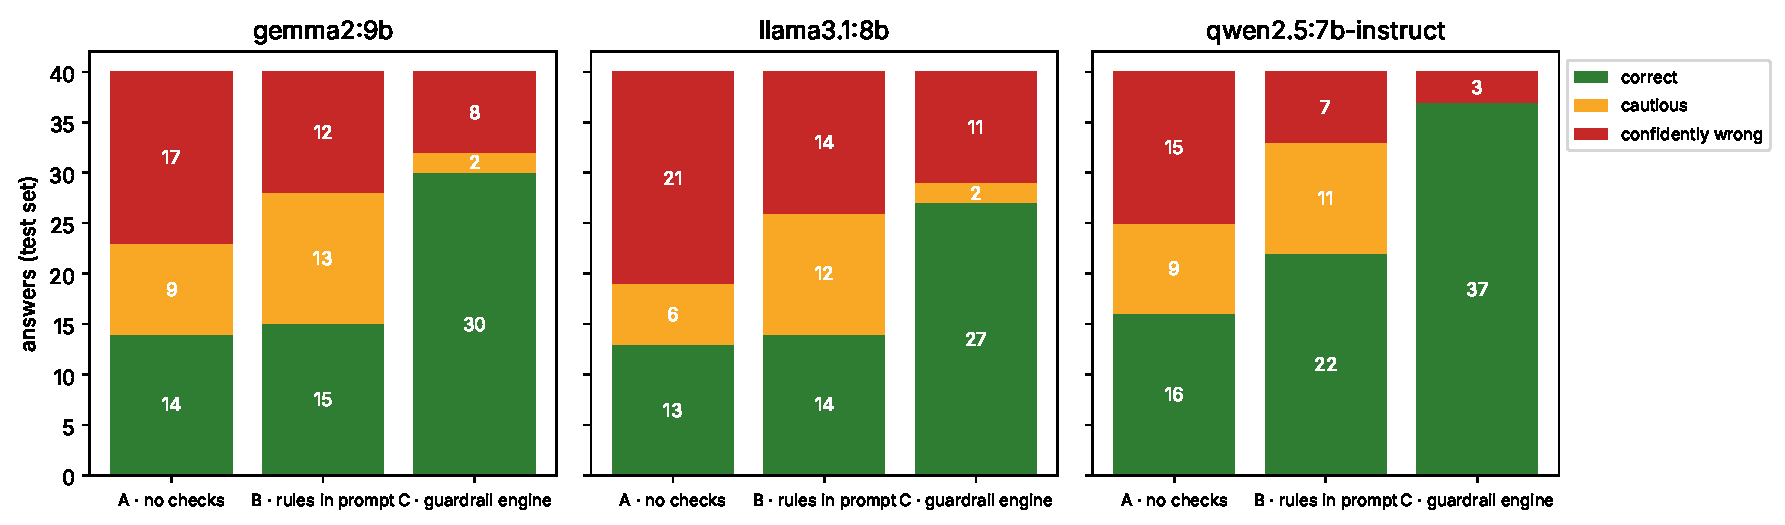
\includegraphics[width=0.8\textwidth]{fig_main.pdf}
\caption{Test run T1: 40 sealed questions per model and setup. Bars split each setup's answers into correct (green), cautious (yellow) and confidently wrong (red).}
\label{fig:main}
\end{figure*}

\begin{table}[t]
\caption{T1 results on the 40 sealed questions (correct / cautious / confidently wrong) and paired tests of C against B}
\label{tab:t1}
\centering\small
\begin{tabular}{@{}lcccc@{}}
\toprule
Model & A & B & C & $p_\text{Holm}$ H2 / H1 \\
\midrule
Qwen 2.5 7B  & 16/9/15 & 22/11/7  & \textbf{37/0/3} & 0.0004 / 0.52 \\
Llama 3.1 8B & 13/6/21 & 14/12/14 & \textbf{27/2/11} & 0.0022 / 0.52 \\
Gemma 2 9B   & 14/9/17 & 15/13/12 & \textbf{30/2/8} & 0.0007 / 0.52 \\
\bottomrule
\end{tabular}
\end{table}

\emph{Main result.} Code-enforced checks roughly double the number of correct answers compared with the same rules in the prompt, for all three model families (Fig.~\ref{fig:main}, Table~\ref{tab:t1}; H2 holds for every model). Qwen reaches 92\,\% correct (Wilson CI 80--97\,\%), above the 90\,\% target set in the proposal; Llama and Gemma reach 68\,\% and 75\,\%. Confidently wrong answers fall for every model (7$\to$3, 14$\to$11, 12$\to$8), but with 40 paired questions the reduction is not significant (one-sided $p$ = 0.17--0.27 before correction), so H1 is not supported. The proposal target of at most 2\,\% confidently wrong is not met (Qwen: 8\,\%).

\begin{figure}[t]
\centering
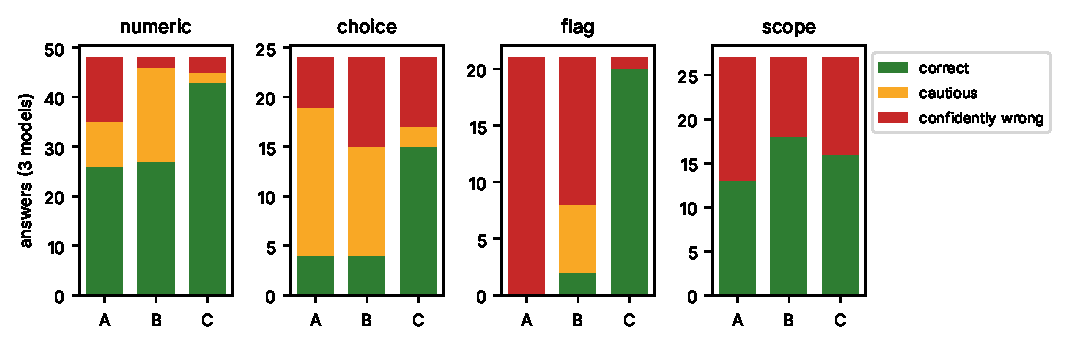
\includegraphics[width=\columnwidth]{fig_types.pdf}
\caption{T1 answers by question type, summed over the three models (A: no checks, B: prompt rules, C: code checks).}
\label{fig:types}
\end{figure}

\emph{By question type} (Fig.~\ref{fig:types}). The gain concentrates where the rule is a computation or a code: flag questions go from 2/21 correct (B) to 20/21 (C), because the validity warning is set by code; numeric questions from 27/48 to 43/48. Scope questions do not improve (B 18/27, C 16/27): the keyword-based scope check of setup C misses out-of-scope questions phrased without a listed keyword (e.g.\ replacing reach trucks by AGVs, a dispatching rule the model lacks), while the prompt rules let the LLM judge the meaning. One numeric question asking for units per \emph{hour} was answered with the per-\emph{shift} value by all three models in C; the value check passes because the number did come from the simulator.

\emph{Repeats and development rerun.} At temperature 0.7 (T2, three seeds) Qwen in C answers 35, 37 and 35 of 40 correctly, against 15--23 in B and 16--18 in A, so the ordering C~$>$~B~$>$~A is stable under sampling. Rerunning Llama on the 80 development questions on the Windows workstation gives 64/8/8 in C, close to the 63/10/7 measured earlier on a cloud GPU.

\emph{Ablation} (T3). Switching off one check at a time in setup C (Qwen, Table~\ref{tab:abl}) shows which checks carry the result on this test set. Without the validity check all seven flag questions become confidently wrong; without adaptive replications a single run replaces the confidence interval and correct answers drop from 37 to 28, mostly on numeric and choice questions; without the scope check three more out-of-scope questions are answered. Switching off the unit, paired-comparison or value check changes no answer: no test question needed a unit conversion of an input, and the paired verdicts were already clear without common random numbers.

\begin{table}[t]
\caption{Ablation (T3): Qwen 2.5 7B, setup C with one check off}
\label{tab:abl}
\centering\small
\begin{tabular}{@{}lccc@{}}
\toprule
Check switched off & correct & cautious & conf.\ wrong \\
\midrule
none (all checks on) & 37 & 0 & 3 \\
validity & 30 & 0 & 10 \\
adaptive replications & 28 & 4 & 8 \\
scope & 34 & 0 & 6 \\
units & 37 & 0 & 3 \\
paired comparison & 37 & 0 & 3 \\
value check & 37 & 0 & 3 \\
\bottomrule
\end{tabular}
\end{table}


\section{Discussion and Limitations}
The results support the LLM-Modulo view \cite{kambhampati2024} for numerical simulation work: the same rules help little as prompt text but substantially as code, and a 7B model with code checks reaches the accuracy target. The ablation confirms that the validity check and adaptive replications carry most of the gain, both of which need no understanding of language; the one that relies on matching words (scope) is the weakest part of the system. A semantic scope check, for example comparing the question with the case card's \texttt{cannot\_answer} list, and a unit check on the final answer are the next steps.

Threats to validity: (i) 40 questions are too few to show a significant drop in confidently wrong answers; (ii) the test questions were written by the system's author, although only after the freeze, by script, with hashed files; (iii) A1 answers come from stored runs of the four published scenarios; (iv) one grader script decides all outcomes, but it was frozen before the test and is public; (v) all models are 7--9B open-weight models run with Ollama defaults.

\section{Conclusion}
Moving simulation methodology from the prompt into code lets small local language models operate validated production simulation models correctly in most cases, on questions none of the rules were tuned on. Future work adds a fifth model from a further industry (a steel-works transport model built in AnyLogic and validated against one year of operating data), a semantic scope check, and a larger question set to test the reduction of confidently wrong answers with adequate power. Code, case cards, questions, protocol and all answers: \url{https://github.com/bodhi584/planner-copilot-guardrails}.

\begin{thebibliography}{99}
\bibitem{law2015} A.~M. Law, \emph{Simulation Modeling and Analysis}, 5th~ed. New York, NY, USA: McGraw-Hill, 2015.
\bibitem{sargent2013} R.~G. Sargent, ``Verification and validation of simulation models,'' \emph{J. Simulation}, vol.~7, no.~1, pp.~12--24, 2013.
\bibitem{kambhampati2024} S.~Kambhampati \emph{et al.}, ``Position: LLMs can't plan, but can help planning in LLM-Modulo frameworks,'' in \emph{Proc. 41st Int. Conf. Machine Learning (ICML)}, PMLR vol.~235, 2024, pp.~22895--22907.
\bibitem{schmitt2026} T.~Schmitt, N.~Gegenmantel, M.~Urenda Moris, P.~M{\aa}rtensson, and K.~Amouzgar, ``LLM-driven discrete-event simulation: A generative AI framework for automated model generation, adaptation, and evaluation in manufacturing,'' \emph{J. Manuf. Syst.}, vol.~85, pp.~642--661, 2026, doi: 10.1016/j.jmsy.2026.02.015.
\bibitem{korth2026} M.~Korth \emph{et al.}, ``LLM-supported usage of simulation and optimization in production planning and control,'' \emph{Simulation Notes Europe}, vol.~36, no.~3, pp.~139--146, 2026, doi: 10.11128/sne.36.tn.10784.
\bibitem{agenticdes2026} ``Agentic discrete-event simulation for manufacturing system design: an open 3D simulator, a benchmark and an industrial case,'' arXiv:2611.10602, 2026.
\bibitem{rebedea2023} T.~Rebedea, R.~Dinu, M.~N. Sreedhar, C.~Parisien, and J.~Cohen, ``NeMo Guardrails: A toolkit for controllable and safe LLM applications with programmable rails,'' in \emph{Proc. EMNLP: System Demonstrations}, 2023, pp.~431--445, doi: 10.18653/v1/2023.emnlp-demo.40.
\bibitem{kopp2020} D.~Kopp \emph{et al.}, ``SMT2020---A semiconductor manufacturing testbed,'' \emph{IEEE Trans. Semicond. Manuf.}, 2020, doi: 10.1109/TSM.2020.3001933.
\bibitem{tassel2023} P.~Tassel, B.~Kov{\'a}cs, M.~Gebser, K.~Schekotihin, P.~St{\"o}ckermann, and G.~Seidel, ``Semiconductor fab scheduling with self-supervised and reinforcement learning,'' arXiv:2302.07162, 2023.
\bibitem{jurczyk2026} M.~Jurczyk-Bunkowska, ``JaamSim models, order portfolios, and replication results for capacity planning in an SME manufacturing system,'' Zenodo, 2026, doi: 10.5281/zenodo.23229885.
\bibitem{saengphueng2026} Saengphueng, ``Code and data for: Task interleaving in warehouse operations,'' Zenodo, 2026, doi: 10.5281/zenodo.21469786.
\bibitem{seppanen2005} M.~S. Seppanen, ``Operator-paced assembly line simulation,'' in \emph{Proc. Winter Simulation Conf.}, 2005, pp.~1343--1349, doi: 10.1109/WSC.2005.1574396.
\bibitem{mcnemar1947} Q.~McNemar, ``Note on the sampling error of the difference between correlated proportions or percentages,'' \emph{Psychometrika}, vol.~12, no.~2, pp.~153--157, 1947.
\bibitem{holm1979} S.~Holm, ``A simple sequentially rejective multiple test procedure,'' \emph{Scand. J. Statist.}, vol.~6, no.~2, pp.~65--70, 1979.
\bibitem{wilson1927} E.~B. Wilson, ``Probable inference, the law of succession, and statistical inference,'' \emph{J. Amer. Statist. Assoc.}, vol.~22, no.~158, pp.~209--212, 1927.
\end{thebibliography}

\end{document}
